\documentclass[12pt, a4]{article}
\usepackage[english]{babel}
\usepackage[utf8x]{inputenc}
\usepackage{fullpage}
\usepackage{listings}
\usepackage{graphicx}
\usepackage{color}

%Syntax highlighting
\definecolor{blue-violet}{rgb}{0.54, 0.17, 0.89}
\definecolor{ao}{rgb}{0.0, 0.5, 0.0}
\definecolor{amaranth}{rgb}{0.9, 0.17, 0.31}
\definecolor{ballblue}{rgb}{0.13, 0.67, 0.8}
\definecolor{onyx}{rgb}{0.06, 0.06, 0.06}


\lstset{
  breaklines=true,                 % automatic line breaking only at whitespace
  captionpos=b,                    % sets the caption-position to bottom
  breakatwhitespace=false,
  keepspaces=true,
  numbers=left,
  numbersep=5pt,
  showspaces=false,
  showstringspaces=false,
  showtabs=false,
  tabsize=4,  
  backgroundcolor=\color{white},   % choose the background color
  commentstyle=\color{ao},    % comment style
  keywordstyle=\color{amaranth},    % keyword style
  stringstyle=\color{blue-violet},    % string literal style
  numberstyle=\tiny\color{ballblue},	   % number style
  basicstyle=\ttfamily\footnotesize\color{onyx} % size of fonts used for the code
}

%Document Header
\title{\textbf{Department of CSE\\SSN College of Engineering}}
\author{\textbf{Vishakan Subramanian - 18 5001 196 - Semester VII}}
\date{02 August 2021}

\begin{document}
\maketitle
\hrule
\section*{\center{UCS 1711 - Mobile Application Development Lab}}
\hrule
\bigskip

%Assignment Details
\subsection*{\center{\textbf{Exercise 2: Application For Calculator and Keyboard Simulation}}}
\subsection*{\flushleft{Aim:}}
\begin{flushleft}
To develop an Android application that performs the functions of a basic calculator and also to develop a custom keyboard to accept numeric input from the user.

\end{flushleft}

%Code
\newpage
\subsection*{\flushleft{Code: Main Activity:}}
\begin{flushleft}
\lstinputlisting[language = Java]{Calculator/app/src/main/java/com/example/calculator/MainActivity.java}
\end{flushleft}

%Code
\newpage
\subsection*{\flushleft{Code: MyInputMethodService:}}
\begin{flushleft}
\lstinputlisting[language = Java]{Calculator/app/src/main/java/com/example/calculator/MyInputMethodService.java}
\end{flushleft}

%Code
\newpage
\subsection*{\flushleft{Code: Main Activity Layout}}
\begin{flushleft}
\lstinputlisting[language = XML]{Calculator/app/src/main/res/layout/activity_main.xml}
\end{flushleft}

%Code
\newpage
\subsection*{\flushleft{Code: Keyboard View Layout}}
\begin{flushleft}
\lstinputlisting[language = XML]{Calculator/app/src/main/res/layout/keyboard_view.xml}
\end{flushleft}

%Code
\newpage
\subsection*{\flushleft{Code: Key Preview Layout}}
\begin{flushleft}
\lstinputlisting[language = XML]{Calculator/app/src/main/res/layout/key_preview.xml}
\end{flushleft}

%Code
\newpage
\subsection*{\flushleft{Code: Method XML}}
\begin{flushleft}
\lstinputlisting[language = XML]{Calculator/app/src/main/res/xml/method.xml}
\end{flushleft}

%Code
\newpage
\subsection*{\flushleft{Code: Number Pad XML}}
\begin{flushleft}
\lstinputlisting[language = XML]{Calculator/app/src/main/res/xml/number_pad.xml}
\end{flushleft}

%Code
\newpage
\subsection*{\flushleft{Code: Android Manifest}}
\begin{flushleft}
\lstinputlisting[language = XML]{Calculator/app/src/main/AndroidManifest.xml}
\end{flushleft}

%Output
\newpage
\subsection*{\flushleft{Output: Calculator Input 1:}}
\begin{figure}[h]
\centering
\caption{Output: Calculator Input 1.}
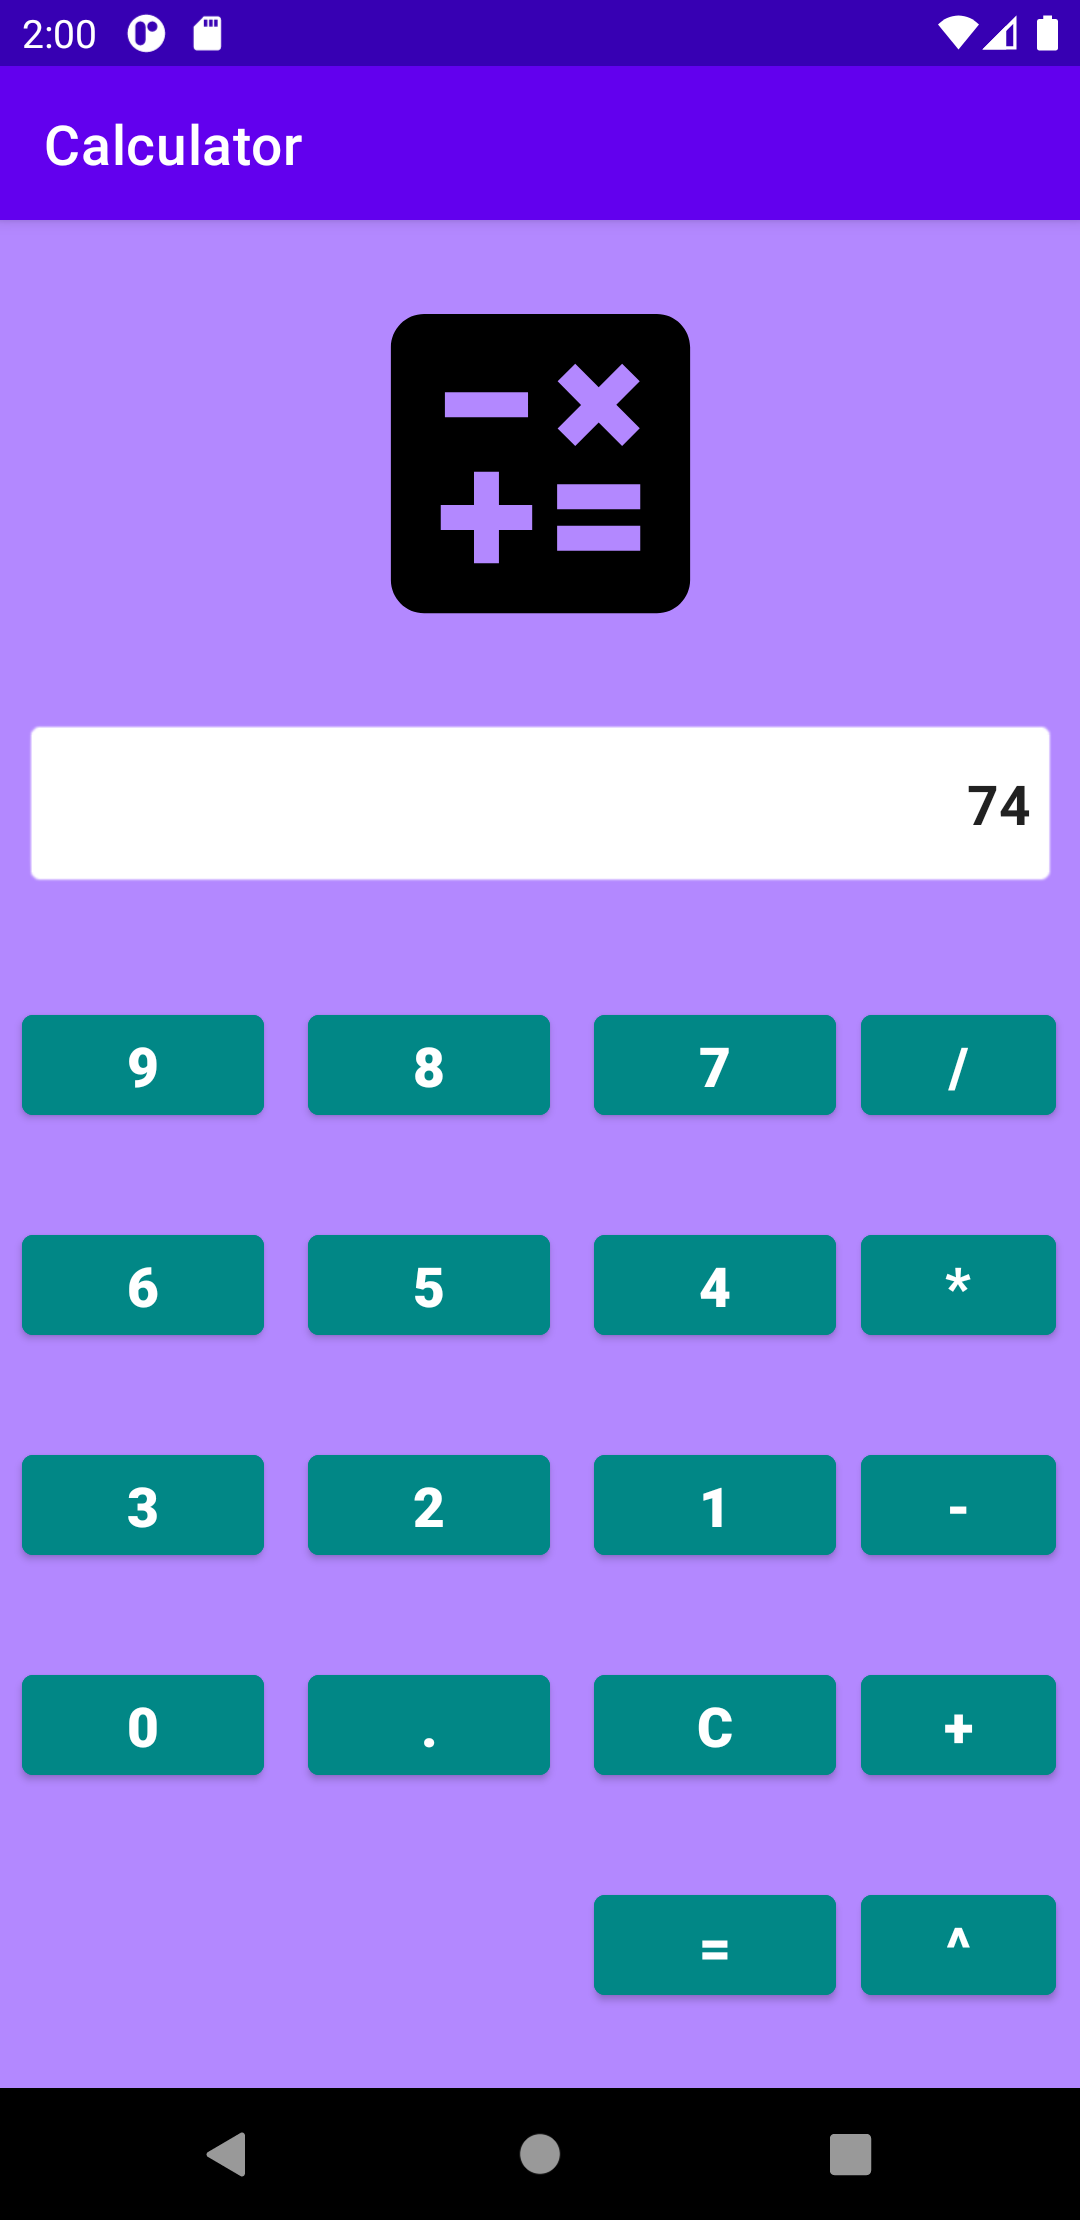
\includegraphics[height=15cm, width=7.3cm]{Calculator/Screenshots/Calculator-1.png}
\end{figure}

%Output
\newpage
\subsection*{\flushleft{Output: Calculator Input 2:}}
\begin{figure}[h]
\centering
\caption{Output: Calculator Input 2.}
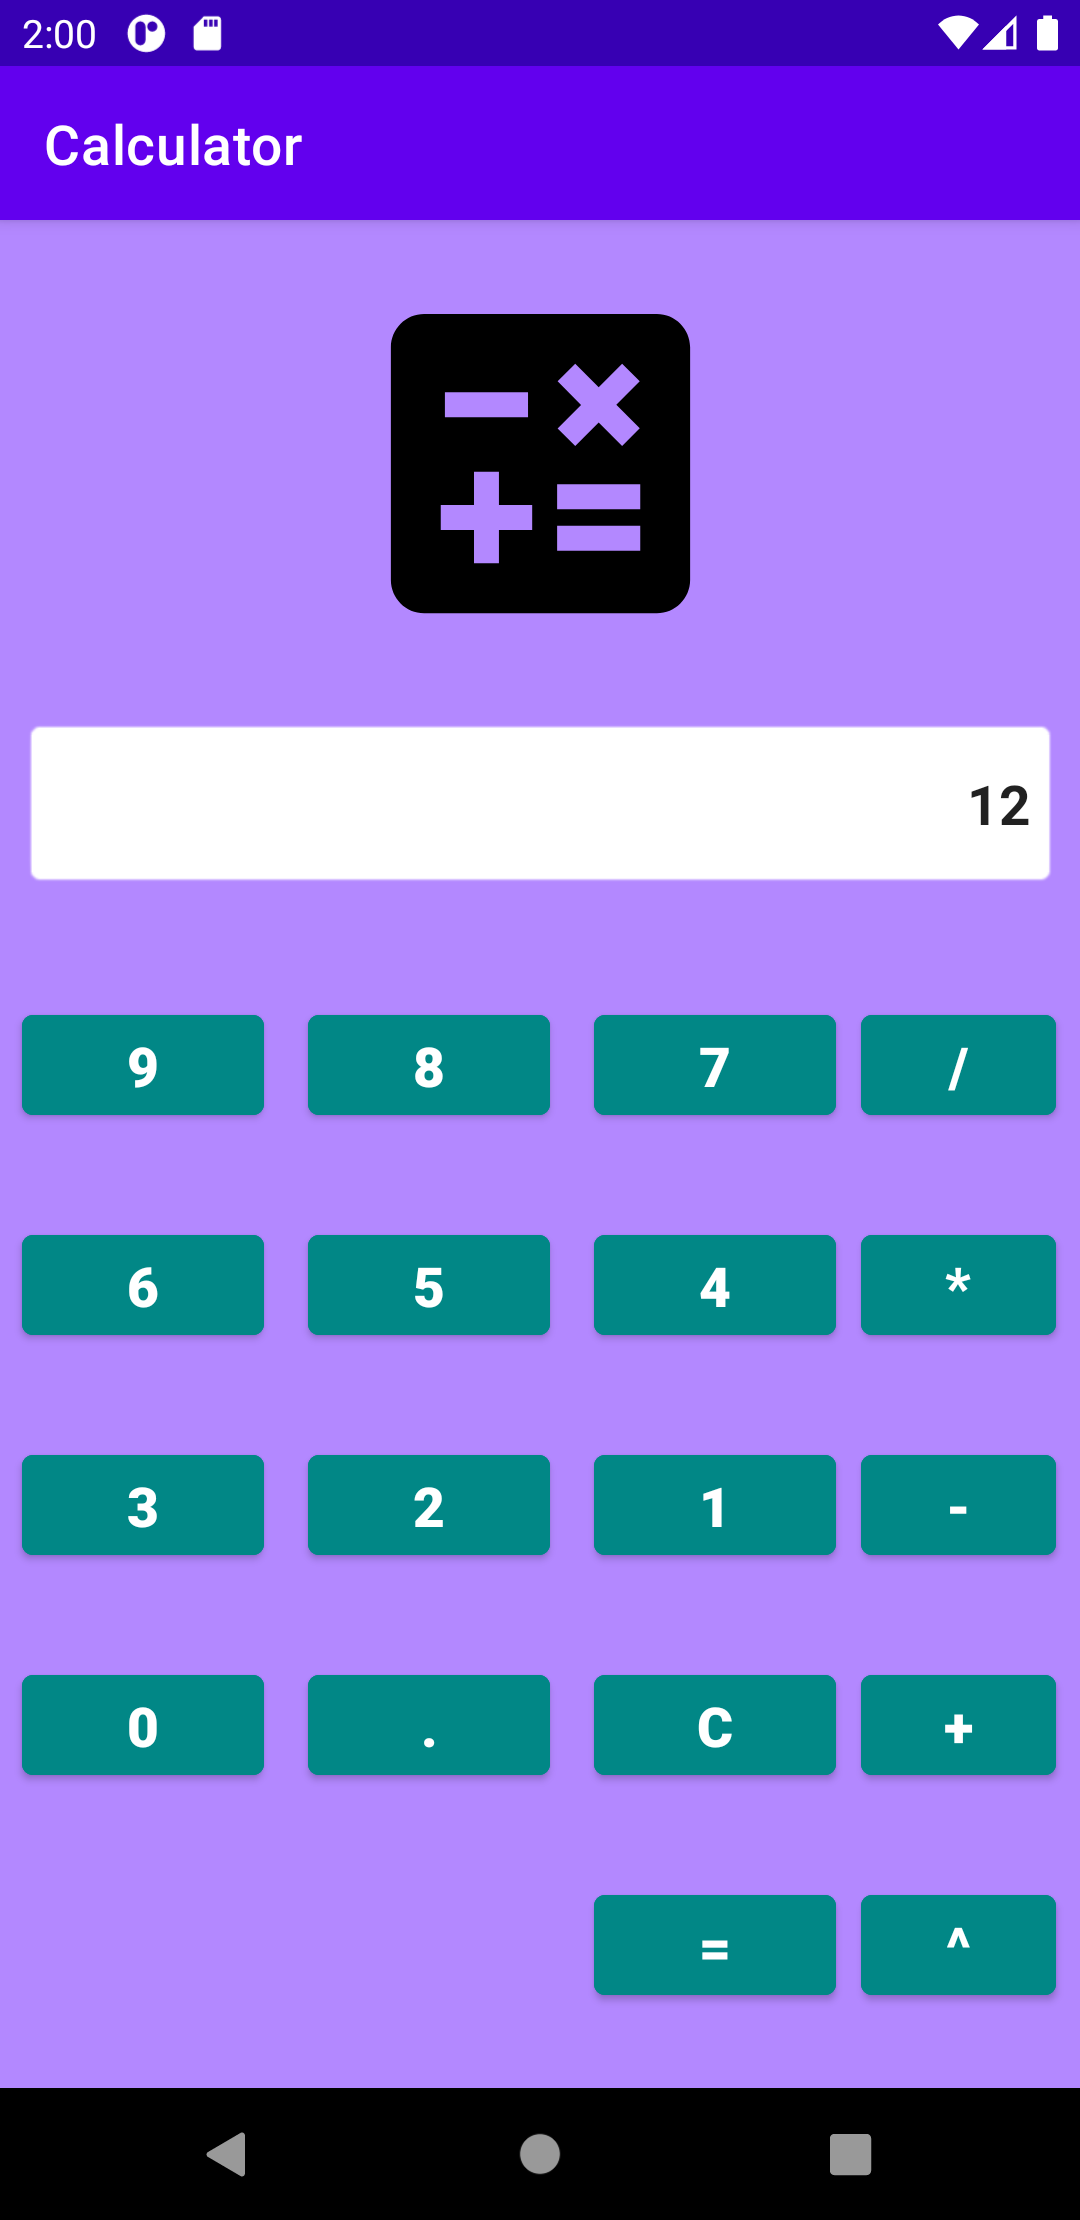
\includegraphics[height=15cm, width=7.3cm]{Calculator/Screenshots/Calculator-2.png}
\end{figure}

%Output
\newpage
\subsection*{\flushleft{Output: Calculator Result:}}
\begin{figure}[h]
\centering
\caption{Output: Calculator Result.}
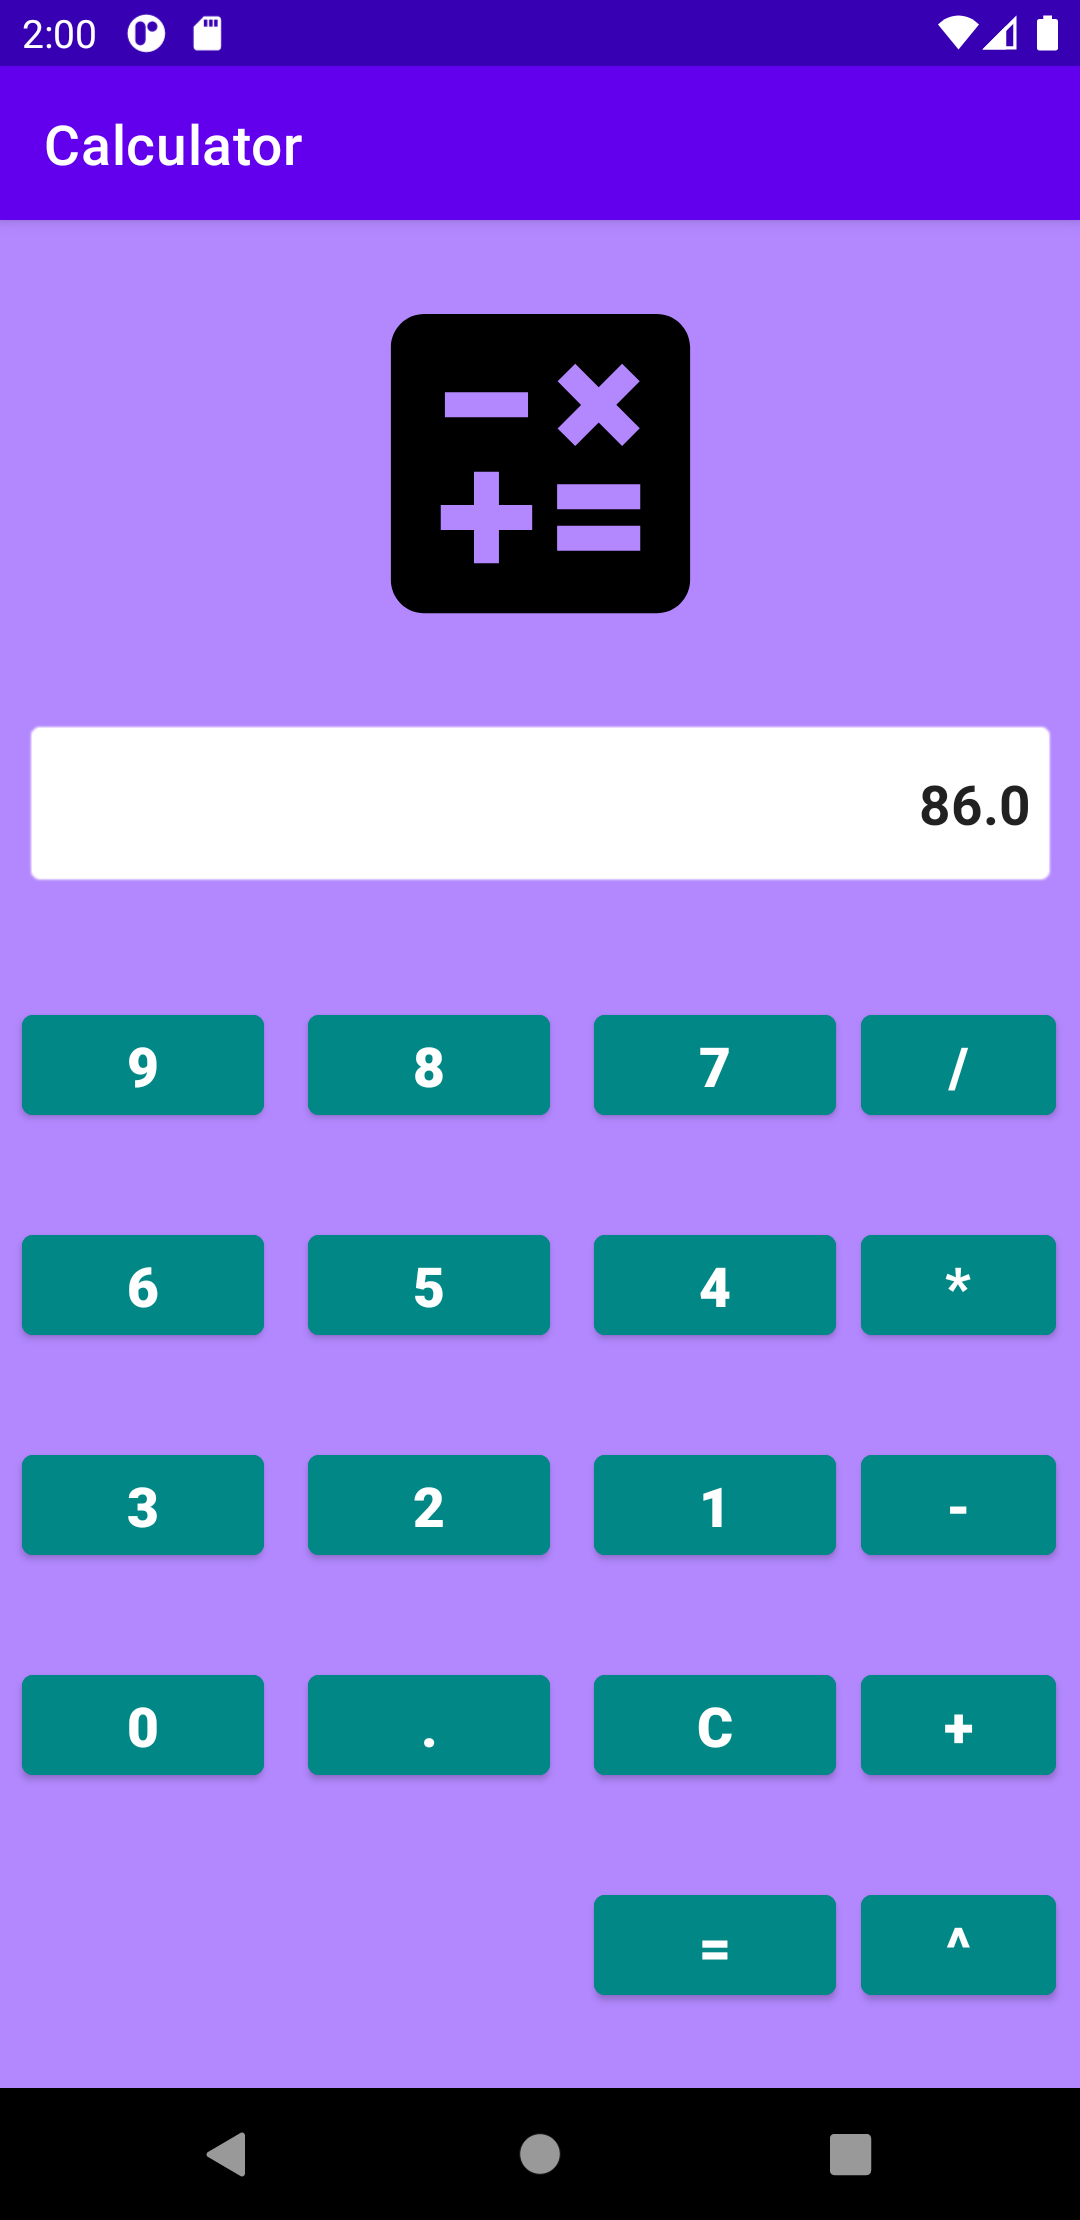
\includegraphics[height=15cm, width=7.3cm]{Calculator/Screenshots/Calculator-3.png}
\end{figure}

%Output
\newpage
\subsection*{\flushleft{Output: Custom Keyboard Set-Up:}}
\begin{figure}[h]
\centering
\caption{Output: Custom Keyboard Set-Up.}
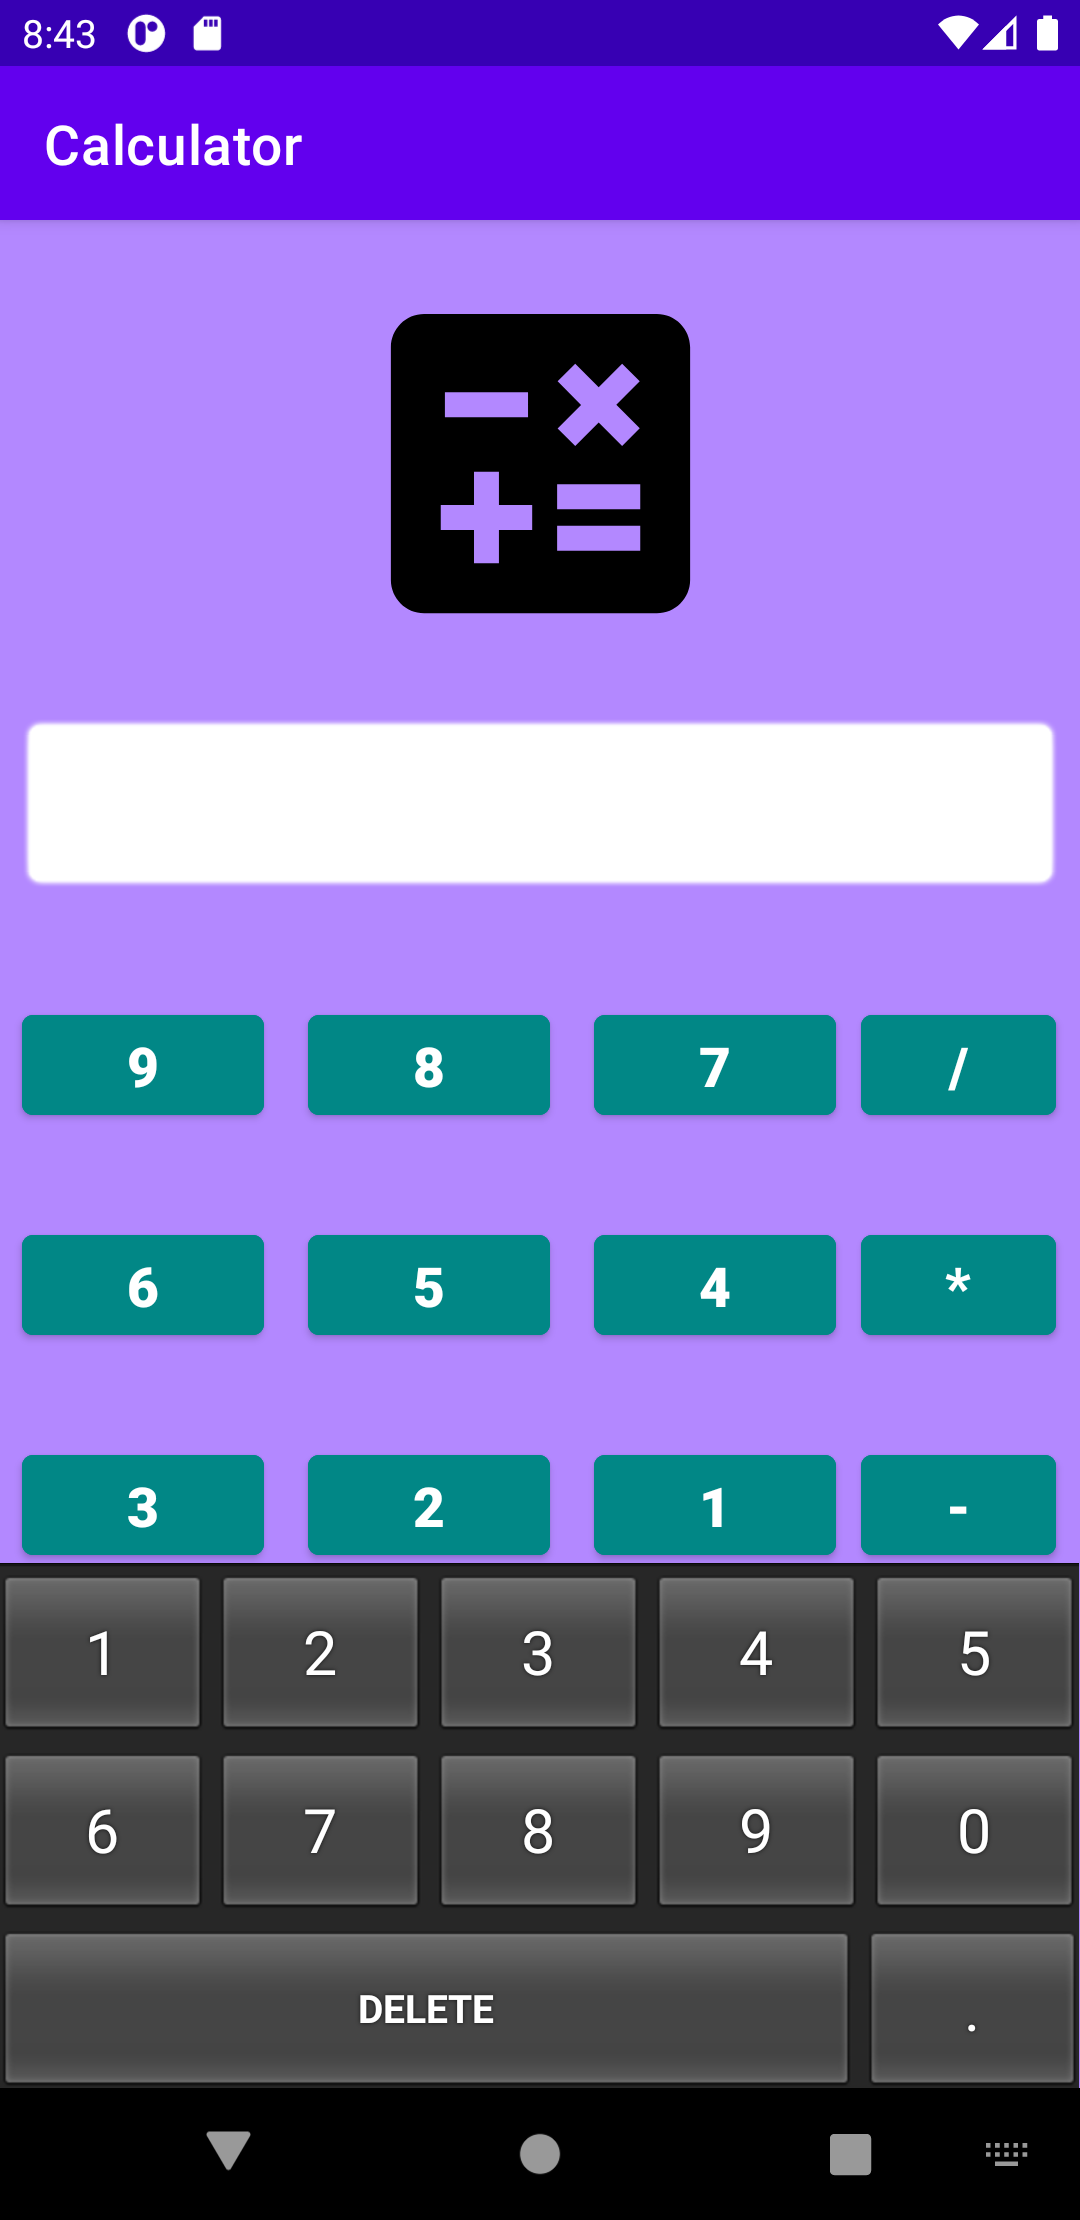
\includegraphics[height=15cm, width=7.3cm]{Calculator/Screenshots/Calculator-4.png}
\end{figure}

%Output
\newpage
\subsection*{\flushleft{Output: Custom Keyboard In Use:}}
\begin{figure}[h]
\centering
\caption{Output: Custom Keyboard In Use.}
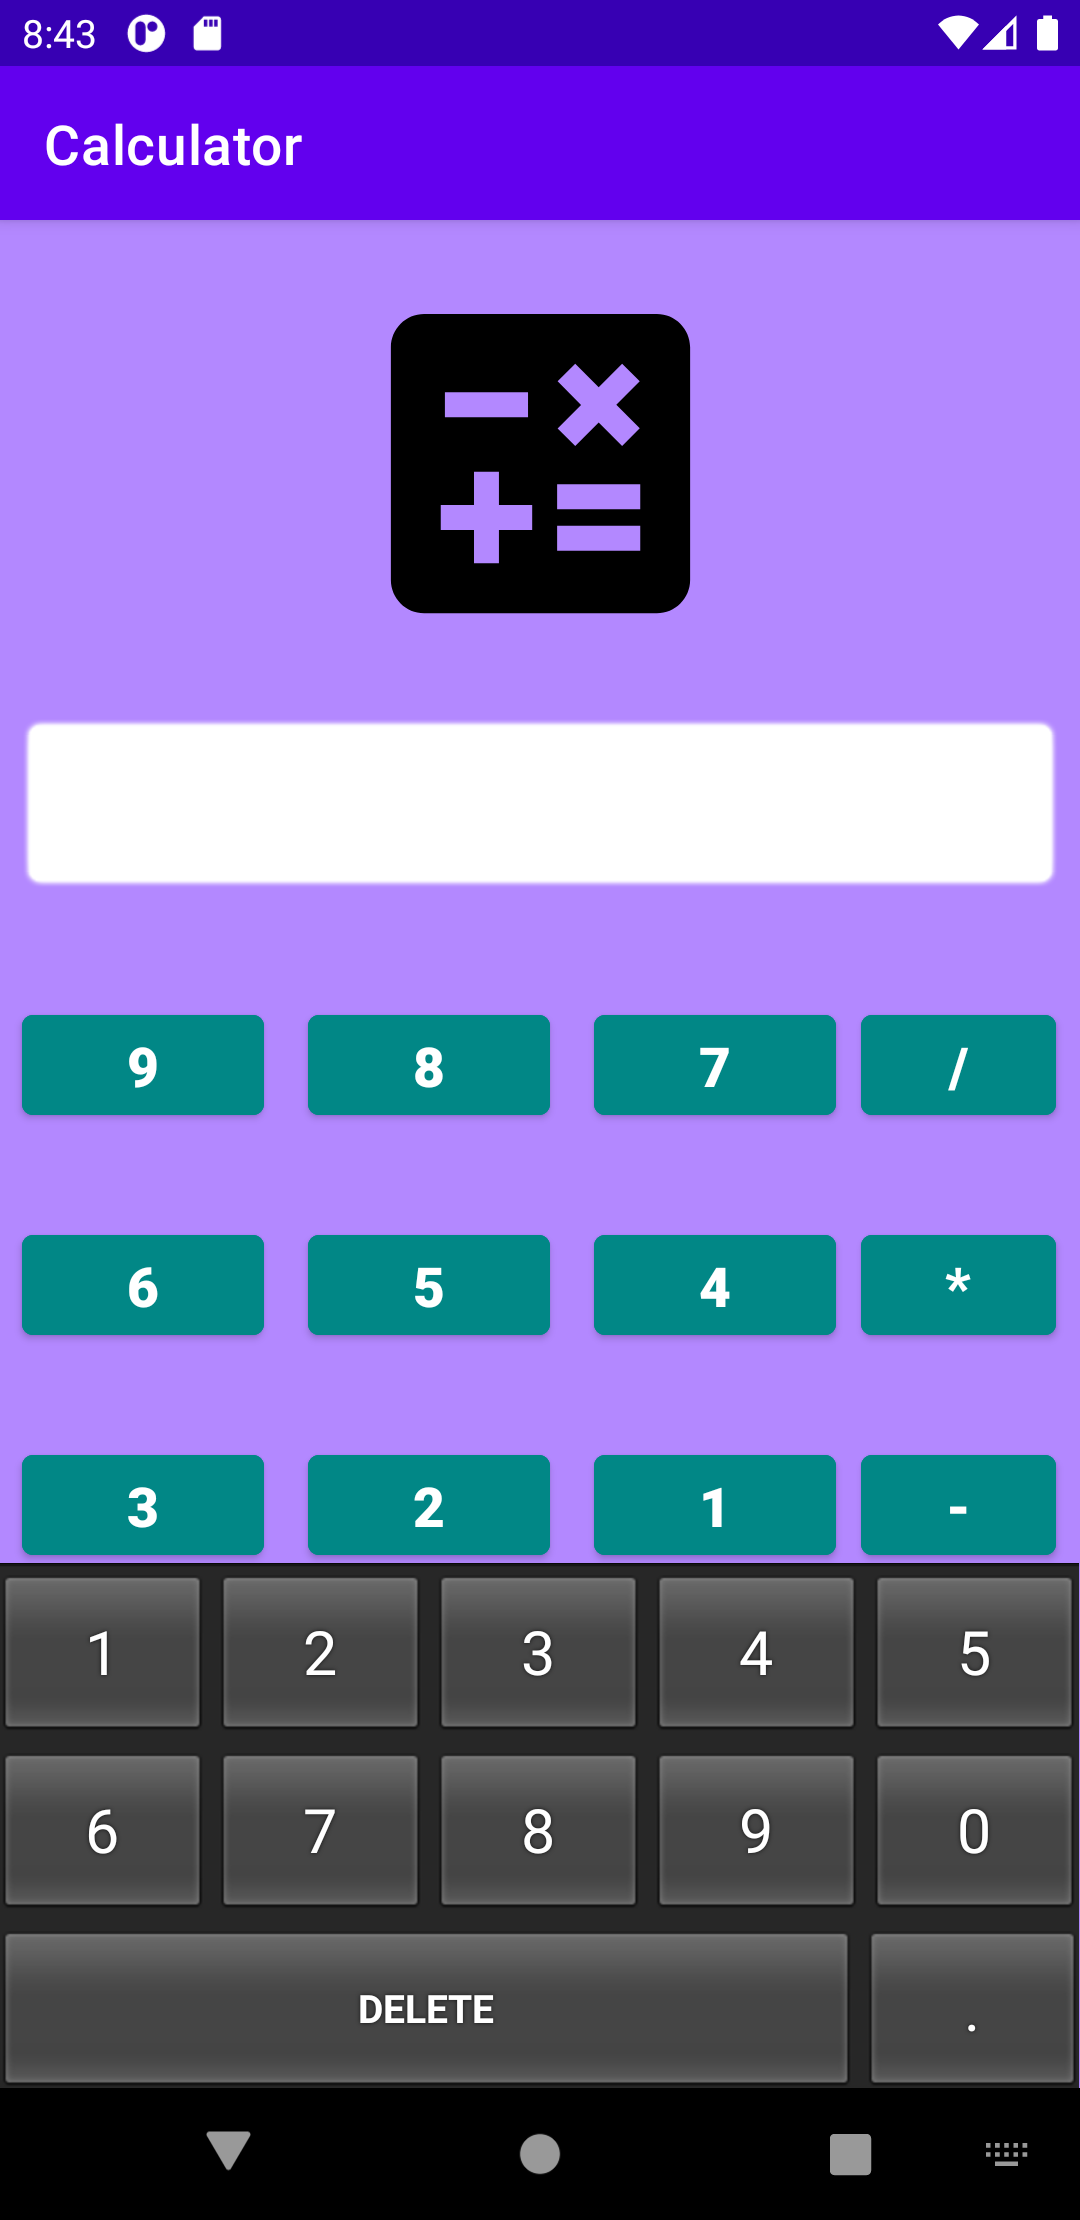
\includegraphics[height=15cm, width=7.3cm]{Calculator/Screenshots/Calculator-5.png}
\end{figure}

%Learning Outcome
\newpage
\subsection*{\flushleft{Learning Outcome:}}
\begin{itemize}
\item I understood how to set-up a layout for a simple calculator application.
\item I implemented the calculator logic with appropriate display functionality.
\item I implemented buttons with logic for clearing the display area and include decimal points as well.
\item I understood how to design a \textbf{custom keyboard} for Android.
\item I understood how to map the keyboard keys to appropriate actions using the \textbf{InputMethodService class \& OnKeyboardActionListener interface}.
\item I implemented functionality to clear the screen using a keypress as well.
\item I understood how to style my custom keyboard using XML.
\item I understood how to add keys to the custom keyboard using XML definition.
\item I learnt that the keyboard service must be exposed to the device through the \textbf{Android Manifest} XML file for end-user peruse.
\item I understood how to enable the custom keyboard from the front-end layer of the Android device.
\end{itemize}


\end{document}